% Options for packages loaded elsewhere
% Options for packages loaded elsewhere
\PassOptionsToPackage{unicode}{hyperref}
\PassOptionsToPackage{hyphens}{url}
\PassOptionsToPackage{dvipsnames,svgnames,x11names}{xcolor}
%
\documentclass[
  spanish,
  letterpaper,
  DIV=11,
  numbers=noendperiod]{scrartcl}
\usepackage{xcolor}
\usepackage[left=2.54cm,right=2.54cm,top=2.54cm,bottom=2.54cm]{geometry}
\usepackage{amsmath,amssymb}
\setcounter{secnumdepth}{-\maxdimen} % remove section numbering
\usepackage{iftex}
\ifPDFTeX
  \usepackage[T1]{fontenc}
  \usepackage[utf8]{inputenc}
  \usepackage{textcomp} % provide euro and other symbols
\else % if luatex or xetex
  \usepackage{unicode-math} % this also loads fontspec
  \defaultfontfeatures{Scale=MatchLowercase}
  \defaultfontfeatures[\rmfamily]{Ligatures=TeX,Scale=1}
\fi
\usepackage{lmodern}
\ifPDFTeX\else
  % xetex/luatex font selection
\fi
% Use upquote if available, for straight quotes in verbatim environments
\IfFileExists{upquote.sty}{\usepackage{upquote}}{}
\IfFileExists{microtype.sty}{% use microtype if available
  \usepackage[]{microtype}
  \UseMicrotypeSet[protrusion]{basicmath} % disable protrusion for tt fonts
}{}
\usepackage{setspace}
\makeatletter
\@ifundefined{KOMAClassName}{% if non-KOMA class
  \IfFileExists{parskip.sty}{%
    \usepackage{parskip}
  }{% else
    \setlength{\parindent}{0pt}
    \setlength{\parskip}{6pt plus 2pt minus 1pt}}
}{% if KOMA class
  \KOMAoptions{parskip=half}}
\makeatother
% Make \paragraph and \subparagraph free-standing
\makeatletter
\ifx\paragraph\undefined\else
  \let\oldparagraph\paragraph
  \renewcommand{\paragraph}{
    \@ifstar
      \xxxParagraphStar
      \xxxParagraphNoStar
  }
  \newcommand{\xxxParagraphStar}[1]{\oldparagraph*{#1}\mbox{}}
  \newcommand{\xxxParagraphNoStar}[1]{\oldparagraph{#1}\mbox{}}
\fi
\ifx\subparagraph\undefined\else
  \let\oldsubparagraph\subparagraph
  \renewcommand{\subparagraph}{
    \@ifstar
      \xxxSubParagraphStar
      \xxxSubParagraphNoStar
  }
  \newcommand{\xxxSubParagraphStar}[1]{\oldsubparagraph*{#1}\mbox{}}
  \newcommand{\xxxSubParagraphNoStar}[1]{\oldsubparagraph{#1}\mbox{}}
\fi
\makeatother


\usepackage{longtable,booktabs,array}
\usepackage{calc} % for calculating minipage widths
% Correct order of tables after \paragraph or \subparagraph
\usepackage{etoolbox}
\makeatletter
\patchcmd\longtable{\par}{\if@noskipsec\mbox{}\fi\par}{}{}
\makeatother
% Allow footnotes in longtable head/foot
\IfFileExists{footnotehyper.sty}{\usepackage{footnotehyper}}{\usepackage{footnote}}
\makesavenoteenv{longtable}
\usepackage{graphicx}
\makeatletter
\newsavebox\pandoc@box
\newcommand*\pandocbounded[1]{% scales image to fit in text height/width
  \sbox\pandoc@box{#1}%
  \Gscale@div\@tempa{\textheight}{\dimexpr\ht\pandoc@box+\dp\pandoc@box\relax}%
  \Gscale@div\@tempb{\linewidth}{\wd\pandoc@box}%
  \ifdim\@tempb\p@<\@tempa\p@\let\@tempa\@tempb\fi% select the smaller of both
  \ifdim\@tempa\p@<\p@\scalebox{\@tempa}{\usebox\pandoc@box}%
  \else\usebox{\pandoc@box}%
  \fi%
}
% Set default figure placement to htbp
\def\fps@figure{htbp}
\makeatother


% definitions for citeproc citations
\NewDocumentCommand\citeproctext{}{}
\NewDocumentCommand\citeproc{mm}{%
  \begingroup\def\citeproctext{#2}\cite{#1}\endgroup}
\makeatletter
 % allow citations to break across lines
 \let\@cite@ofmt\@firstofone
 % avoid brackets around text for \cite:
 \def\@biblabel#1{}
 \def\@cite#1#2{{#1\if@tempswa , #2\fi}}
\makeatother
\newlength{\cslhangindent}
\setlength{\cslhangindent}{1.5em}
\newlength{\csllabelwidth}
\setlength{\csllabelwidth}{3em}
\newenvironment{CSLReferences}[2] % #1 hanging-indent, #2 entry-spacing
 {\begin{list}{}{%
  \setlength{\itemindent}{0pt}
  \setlength{\leftmargin}{0pt}
  \setlength{\parsep}{0pt}
  % turn on hanging indent if param 1 is 1
  \ifodd #1
   \setlength{\leftmargin}{\cslhangindent}
   \setlength{\itemindent}{-1\cslhangindent}
  \fi
  % set entry spacing
  \setlength{\itemsep}{#2\baselineskip}}}
 {\end{list}}
\usepackage{calc}
\newcommand{\CSLBlock}[1]{\hfill\break\parbox[t]{\linewidth}{\strut\ignorespaces#1\strut}}
\newcommand{\CSLLeftMargin}[1]{\parbox[t]{\csllabelwidth}{\strut#1\strut}}
\newcommand{\CSLRightInline}[1]{\parbox[t]{\linewidth - \csllabelwidth}{\strut#1\strut}}
\newcommand{\CSLIndent}[1]{\hspace{\cslhangindent}#1}

\ifLuaTeX
\usepackage[bidi=basic]{babel}
\else
\usepackage[bidi=default]{babel}
\fi
% get rid of language-specific shorthands (see #6817):
\let\LanguageShortHands\languageshorthands
\def\languageshorthands#1{}


\setlength{\emergencystretch}{3em} % prevent overfull lines

\providecommand{\tightlist}{%
  \setlength{\itemsep}{0pt}\setlength{\parskip}{0pt}}



 


\usepackage{booktabs}
\usepackage{longtable}
\usepackage{array}
\usepackage{multirow}
\usepackage{wrapfig}
\usepackage{float}
\usepackage{colortbl}
\usepackage{pdflscape}
\usepackage{tabu}
\usepackage{threeparttable}
\usepackage{threeparttablex}
\usepackage[normalem]{ulem}
\usepackage{makecell}
\usepackage{xcolor}
\KOMAoption{captions}{tableheading}
\makeatletter
\@ifpackageloaded{caption}{}{\usepackage{caption}}
\AtBeginDocument{%
\ifdefined\contentsname
  \renewcommand*\contentsname{Tabla de contenidos}
\else
  \newcommand\contentsname{Tabla de contenidos}
\fi
\ifdefined\listfigurename
  \renewcommand*\listfigurename{Listado de Figuras}
\else
  \newcommand\listfigurename{Listado de Figuras}
\fi
\ifdefined\listtablename
  \renewcommand*\listtablename{Listado de Tablas}
\else
  \newcommand\listtablename{Listado de Tablas}
\fi
\ifdefined\figurename
  \renewcommand*\figurename{Figura}
\else
  \newcommand\figurename{Figura}
\fi
\ifdefined\tablename
  \renewcommand*\tablename{Tabla}
\else
  \newcommand\tablename{Tabla}
\fi
}
\@ifpackageloaded{float}{}{\usepackage{float}}
\floatstyle{ruled}
\@ifundefined{c@chapter}{\newfloat{codelisting}{h}{lop}}{\newfloat{codelisting}{h}{lop}[chapter]}
\floatname{codelisting}{Listado}
\newcommand*\listoflistings{\listof{codelisting}{Listado de Listados}}
\makeatother
\makeatletter
\makeatother
\makeatletter
\@ifpackageloaded{caption}{}{\usepackage{caption}}
\@ifpackageloaded{subcaption}{}{\usepackage{subcaption}}
\makeatother
\usepackage{bookmark}
\IfFileExists{xurl.sty}{\usepackage{xurl}}{} % add URL line breaks if available
\urlstyle{same}
\hypersetup{
  pdftitle={Dos décadas de cambios en la cohesión social en América Latina (2004-2023)},
  pdfauthor={Juan Carlos Castillo; Gabriel Cortés Paredes; Andreas Laffert; Kevin Carrasco; Tomás Urzúa},
  pdflang={es},
  pdfkeywords={cohesión social, análisis multinivel, análisis
longitudinal},
  colorlinks=true,
  linkcolor={blue},
  filecolor={Maroon},
  citecolor={Blue},
  urlcolor={Blue},
  pdfcreator={LaTeX via pandoc}}


\title{Dos décadas de cambios en la cohesión social en América Latina
(2004-2023)}
\author{Juan Carlos Castillo \and Gabriel Cortés Paredes \and Andreas
Laffert \and Kevin Carrasco \and Tomás Urzúa}
\date{}
\begin{document}
\maketitle
\begin{abstract}
En un contexto regional marcado por crisis políticas, desigualdades
persistentes y episodios de conflictividad social, comprender la
evolución de la cohesión social es fundamental para evaluar la
estabilidad democrática y la legitimidad institucional. Si bien existen
numerosos estudios sobre las causas y consecuencias de la desconfianza o
la polarización en América Latina, aún persiste un vacío en el análisis
sistemático y longitudinal de la cohesión social como fenómeno integral.
Este proyecto busca llenar ese vacío mediante el desarrollo de un
conjunto de indicadores que permitan analizar con comparabilidad
temporal y regional la evolución de las distintas dimensiones de la
cohesión social.

Este artículo busca cubrir esas brechas proponiendo y validando un
modelo de medición que permita un análisis comparativo, longitudinal y
multinivel de la cohesión social en América Latina. En concreto,
buscamos avanzar en: (i) una operacionalización clara y validada que
integre dimensiones claves a partir de la literatura existente y los
datos disponibles para la región; (ii) la estimación de trayectorias
regionales y nacionales durante las últimas dos décadas; y (iii) la
identificación de factores asociados a estos cambios mediante la
aplicación de modelos de regresión multinivel. Con esto, se espera
aportar evidencia robusta sobre los cambios en la región en las últimas
dos décadas, aportando a la discusión académica y política sobre los
desafíos y oportunidades de la cohesión social en América Latina.
\end{abstract}


\setstretch{1.15}
\section{Introducción}\label{introducciuxf3n}

En América Latina, los últimos años han estado marcadas por episodios de
inestabilidad política, desigualdades persistentes y bajo crecimiento
económico, y ciclos de conflictividad social
(\citeproc{ref-undp_trapped_2023}{United Nations Development Programme
2023}; \citeproc{ref-salazar-xirinachs_repensar_2023}{Salazar-Xirinachs
2023}) . De tal modo, las tensiones sociales parecen haber aumentado en
la región, reflejando una falta de confianza en las instituciones
democráticas y un descontento generalizado con la corrupción y la
desigualdad. En este contexto, la cohesión social ha escalado en la
agenda pública y académica, con diagnósticos recientes tanto de
organismos internacionales como de gobiernos nacionales que advierten
sobre sus tensiones y desafíos para la gobernabilidad democrática y el
desarrollo inclusivo (\citeproc{ref-undp_trapped_2023}{United Nations
Development Programme 2023};
\citeproc{ref-salazar-xirinachs_repensar_2023}{Salazar-Xirinachs 2023};
\citeproc{ref-castillo_cohesion_2022}{Juan Carlos Castillo, Espinoza, y
Barozet 2022}; \citeproc{ref-mideso_informe_2020}{Ministerio de
Desarrollo Social y Familia 2020}).

Sin embargo, pese a su uso generalizado y cotidiano en la discusión
pública, definir cohesión social teórica y operacionalmente sigue siendo
un desafío. La literatura oscila entre estudios focalizados en a una o
varias dimensiones específicas de la cohesión social
(\citeproc{ref-ariely_does_2013}{Ariely 2013};
\citeproc{ref-castillo_cohesion_2022}{Juan Carlos Castillo, Espinoza, y
Barozet 2022}; \citeproc{ref-castillo_social_2023}{Juan Carlos Castillo
et~al. 2023}) a esfuerzos por sintetizar el fenómeno en índices
comprehensivos (\citeproc{ref-langer_conceptualising_2016}{Langer et~al.
2016}; \citeproc{ref-delhey_happier_2016}{Delhey y Dragolov 2016};
\citeproc{ref-delhey_social_2018}{Delhey et~al. 2018};
\citeproc{ref-dragolov_social_2013}{Dragolov et~al. 2013};
\citeproc{ref-janmaat_social_2010}{Janmaat 2010}). Esta heterogeneidad
conceptual y metodológica dificulta la comparación entre países, así
como la detección de transformaciones a lo largo del tiempo.

Por lo demás, la mayoría de estas definiciones se han puesto a prueba
principalmente en países europeos o de altos ingresos
(\citeproc{ref-ariely_does_2013}{Ariely 2013};
\citeproc{ref-delhey_happier_2016}{Delhey y Dragolov 2016}), con solo
menciones parciales a América Latina
(\citeproc{ref-janmaat_social_2010}{Janmaat 2010}). Esta limitación se
mantiene pese a que la evidencia apunta a que las diferencias nacionales
y regionales en los contextos culturales, históricos e institucionales
moldean la cohesión de las sociedades y los factores que la determinan
(\citeproc{ref-janmaat_social_2010}{Janmaat 2010};
\citeproc{ref-delhey_happier_2016}{Delhey y Dragolov 2016}). De tal
modo, pese a la percepción generalizada de que la cohesión social es un
fenómeno en tensión en las sociedades latinoamericanas, existe evidencia
empírica de las diferencias entre países, las tendencias en el tiempo y
los factores que explican estos cambios.

Este artículo busca cubrir esas brechas proponiendo y validando un
modelo de medición que permita un análisis comparativo, longitudinal y
multinivel de la cohesión social en América Latina. En concreto,
buscamos avanzar en: (i) una operacionalización clara y validada que
integre dimensiones claves a partir de la literatura existente y los
datos disponibles para la región; (ii) la estimación de trayectorias
regionales y nacionales durante las últimas dos décadas; y (iii) la
identificación de factores asociados a estos cambios mediante la
aplicación de modelos de regresión multinivel. Con esto, se espera
aportar evidencia robusta sobre los cambios en la región en las últimas
dos décadas, aportando a la discusión académica y política sobre los
desafíos y oportunidades de la cohesión social en América Latina.

\section{¿Qué es la cohesión
social?}\label{quuxe9-es-la-cohesiuxf3n-social}

Aunque sus raíces teóricas se remontan a los inicios de la teoría social
-- y su uso extendido en la discusión pública - definir cohesión social
sigue siendo una tarea difícil
(\citeproc{ref-chan_reconsidering_2006}{Chan, To, y Chan 2006}). Situada
en la intersección entre enfoques teóricos y descriptivos que enfatizan
las cooperación y la integración, y consideraciones normativas acerca de
cómo la sociedades se mantienen unidad ante crisis, tensiones y
transformaciones, la cohesión social se ha definido de múltiples
maneras, reflejando diversas perspectivas, alcances e indicadores
(\citeproc{ref-chan_reconsidering_2006}{Chan, To, y Chan 2006};
\citeproc{ref-castillo_conceptos_2021}{Juan-Carlos Castillo, Olivos, y
Iturra 2021}).

Con todo, la mayoría de las definiciones comparten algunos elementos en
común (\citeproc{ref-castillo_conceptos_2021}{Juan-Carlos Castillo,
Olivos, y Iturra 2021}):

\begin{itemize}
\tightlist
\item
  Es un atributo del colectivo, no de los individuos.
\item
  Es un constructo multidimensional
\item
  Es una cualidad de las relaciones sociales que permite alcanzar fines
  compartidos.
\item
  Dado que los sujetos tiene un objetivo común, son capaces cooperar
  para lograr estos objetivos.
\end{itemize}

Una definición robusta de cohesión social debe integrar estos elementos.
A la vez, debe ser una definición mínima e intuitiva, que permita su
operacionalización y medición, así como la comparación en contextos
diversos y posibilite la discusión e espacios públicos
(\citeproc{ref-chan_reconsidering_2006}{Chan, To, y Chan 2006}).

De tal modo, en este artículo partiremos de la definición propuesta por
Chan, To y Chan (\citeproc{ref-chan_reconsidering_2006}{2006, 90}), para
quienes la cohesión social

\begin{quote}
is a state of affairs concerning both the vertical and the horizontal
interactions among members of society as characterized by a set of
attitudes and norms that includes trust, a sense of belonging and the
willingness to participate and help, as well as their behavioural
manifestations.
\end{quote}

De la definición, pues, se desprenden dos dimensiones principales. En
primer lugar, la cohesión social tiene \textbf{una dimensión
horizontal}. Con esto nos referimos a las interacciones cotidianas entre
los miembros de una sociedad. Contiene aspectos subjetivos (tales como
el sentido de pertenencia y la confianza interpersonal), como aspecto
objetivos, como las redes sociales y las condiciones materiales que
facilitan o dificultan estas interacciones.

En segundo lugar, la cohesión social tiene \textbf{una dimensión
vertical}, que se refiere a las relaciones entre los individuos y las
instituciones sociales y políticas. Esta dimensión incluye aspectos como
la confianza en las instituciones, la legitimidad del sistema político y
la participación cívica.

\section{Tendencias y factores relacionados a la Cohesión
Social}\label{tendencias-y-factores-relacionados-a-la-cohesiuxf3n-social}

Diversos estudios muestran que las trayectorias de la cohesión social
difieren ampliamente entre países. Entre los factores que influyen en
estas trayectorias se cuentan el crecimiento y la desigualdad económica,
la configuración de los sistemas de bienestar, la composición cultural y
étnica, y los legados autoritatorios. La intensidad y la dirección de
sus efectos, sin embargo, dependen en gran medida del contexto. Por
ejemplo, mientras en Europa el crecimiento económico, la igualdad social
y las democracias liberales suelen asociarse con mayores niveles de
cohesión, en varios países de Asia se observan niveles comparables en
contextos de desigualdad moderada y regímenes autoritarios. Ahora bien,
en todos estos estudios las menciones a determinantes de la cohesión
social en sociedades latinoamericanas son escasas.

Con todo, es posible agrupar los factores identificados en tres
dimensiones:

\begin{enumerate}
\def\labelenumi{\arabic{enumi}.}
\tightlist
\item
  Factores socioeconómicos
\item
  Factores institucionales
\item
  Factores culturales
\end{enumerate}

A continuación se revisan cada una de ellas.

\subsection{1) Factores
socioeconómicos}\label{factores-socioeconuxf3micos}

La prosperidad económica, a menudo medida a través del PIB per cápita,
se ha asociado con mayores niveles de cohesión social. Esta asociación
se ha encontrando en diversos contextos culturales
(\citeproc{ref-janmaat_social_2010}{Janmaat 2010};
\citeproc{ref-delhey_social_2023}{Delhey, Dragolov, y Boehnke 2023}),
aunque parece atenuarse en algunas sociedades asiáticas de altos
ingresos (\citeproc{ref-delhey_social_2018}{Delhey et~al. 2018}). Estos
hallazgos van en línea con las perspectivas universalistas o modernistas
de la cohesión social, para quienes la cohesión es un fenómeno
estrechamente relacionado con distintas etapas del desarrollo
socioeconómico (\citeproc{ref-janmaat_social_2010}{Janmaat 2010}). De
estos hallazgos, se desprende la primera hipótesis del artículo:

\begin{quote}
H1(a): Aumentos en el desarrollo económico de un país estarán asociados
con incrementos en los niveles de cohesión social
\end{quote}

\begin{quote}
H1(b): Los países con un mayor desarrollo económico presentarán mayores
niveles de cohesión social
\end{quote}

Por otro lado, la desigualdad económica se ha asociado generalmente con
menores niveles de cohesión social
(\citeproc{ref-delhey_social_2018}{Delhey et~al. 2018};
\citeproc{ref-janmaat_social_2010}{Janmaat 2010}). Nuevamente, sin
embargo, la asociación se atenúa en sociedades asiáticas, donde niveles
medios de desigualdad están asociados con mayores niveles de cohesión
(\citeproc{ref-janmaat_social_2010}{Janmaat 2010};
\citeproc{ref-delhey_social_2018}{Delhey et~al. 2018}).

No hay evidencia sobre como los niveles de desigualdad en América Latina
se relacionan con la cohesión social. Por un lado, pese a ser
considerada una de las regiones más desiguales del mundo, los
latinoamericanos muestran altísimas expectativas de movilidad social
(\citeproc{ref-somma_paradojas_2015}{Somma y Valenzuela 2015}),
posiblemente debido de al aumento de la cobertura educativa en muchos
países de la región o al predominio de las justificaciones
meritocráticas para la desigualdad educativa y
económica(\citeproc{ref-somma_paradojas_2015}{Somma y Valenzuela 2015};
\citeproc{ref-castillo_socialization_2024}{Juan Carlos Castillo et~al.
2024}). Con todo, las demandas de mayor igualdad, redistribución y trato
justo (\citeproc{ref-cabib_nuestras_2025}{Cabib et~al. 2025};
\citeproc{ref-araujo_primer_2022}{Araujo et~al. 2022}), que se han
traducido en protestas masivas en varios países de la región, sugieren
que la desigualdad económica es un factor relevante para la cohesión
social en América Latina. Por lo tanto, planteamos las siguientes
hipótesis:

\begin{quote}
H2(a): Aumentos en la desigualdad económica de un país estarán asociados
con menores niveles de cohesión social
\end{quote}

\begin{quote}
H2(b): Países con mayores niveles de desigualdad presentarán menores
niveles de cohesión social
\end{quote}

\begin{quote}
H3(a): Individuos con mayor nivel educativo mostrarán mayores nivel de
cohesión social
\end{quote}

\begin{quote}
H3(b): El efecto de la desigualdad económica sobre la cohesión social
será menor en países con mayores oportunidades educativas.
\end{quote}

\subsection{2) Factores institucionales}\label{factores-institucionales}

La capacidad del Estado para responder de manera efectiva a las
problemáticas de la población, especialmente de los grupos más
vulnerables, ha sido identificada como una de las principales fuentes de
cohesión social en diversas sociedades
(\citeproc{ref-kustov_diversity_2024}{Kustov y Pardelli 2024};
\citeproc{ref-njozela_measuring_2016}{Njozela, Shaw, y Burns 2016};
\citeproc{ref-andrews_welfare_2015}{ANDREWS y JILKE 2015}). En esta
línea, una gobernanza eficaz y la presencia de instituciones sólidas
suelen asociarse con mayores niveles de cohesión soical en contextos tan
diversos como Asia, América Latina y Europa
(\citeproc{ref-delhey_social_2018}{Delhey et~al. 2018};
\citeproc{ref-green_social_2011}{Green, Janmaat, y Cheng 2011}).

En contraste, la relación entre los sistemas políticos y el régimen
democrático con la cohesión social parece ser más dependiente del
contexto. Mientras que en sociedades occidentales de altos ingresos la
democracia liberal tiende a reforzar los niveles de cohesión social, en
algunos países asiáticos los regímenes autoritarios se han viculado con
niveles igualmente elevados de cohesión
(\citeproc{ref-delhey_social_2018}{Delhey et~al. 2018})

En América Latina, los Estados suelen caracterizarse por menores niveles
de eficiencia y mayores índices de corrupción, acompañados de una
ciudadnaía que presenta bajos niveles de confianza en las instituciones
políticas y una menor participación en comparación con el mundo
desarrollado. Sin embargo, esta desconfianza institucional convive con
un fuerte sentido de identificación nacional, incluso más pronunciado
que en el primer mundo (\citeproc{ref-somma_paradojas_2015}{Somma y
Valenzuela 2015}). Para Somma
(\citeproc{ref-somma_paradojas_2015}{2015}), esta aparente paradoja se
relaciona con la propensión de las sociedades latinoamericanas hacia
liderazgos personalistas y populistas. En este contexto, en línea con lo
que Guillermo O'Donnell describió como democracias delegativas
(\citeproc{ref-toppi_guillermo_2018}{Toppi 2018}), amplios sectores de
la ciudadanía estarían dispuestos a transar principios de la democracia
liberal en favor a liderazgos autoritarios cuando perciben que las
instituciones democráticas no logran resolver sus problemas cotidianos.
Esto sugiere que la efectividad de la gobernanza -- más que el tipo de
régimen político -- es el factor institucional que ejerce un mayor peso
en los niveles de cohesión social en las sociedades latinoamericanas. A
partir de esta discusión, planteamos las siguientes hipótesis:

\begin{quote}
H4(a): Aumentos en los niveles de gobernanza en un país estarán
asociados con mayores niveles de cohesión social
\end{quote}

\begin{quote}
H4(b): Países con mayores niveles de gobernanza presentarán mayores
niveles de cohesión social
\end{quote}

\subsection{3) Factores culturales}\label{factores-culturales}

Las variables culturales y demográficas, incluidas las identidades
étnicas, religiosas y nacionales, han mostrado efectos complejos sobre
niveles de cohesión social, variando sustancialmente según el contexto.
Este carácter contextual es especialmente evidente en el impacto de la
diversidad étnica sobre la cohesión social.

Por un lado, diversos estudios han identificados esfectos negativos de
la diversidad étnica sobre indicadores como el sentido de pertenencia o
la fortaleza de las redes
vecinales(\citeproc{ref-gijsberts_hunkering_2011}{Gijsberts, van der
Meer, y Dagevos 2011}; \citeproc{ref-ariely_does_2013}{Ariely 2013}),
asociación que resulta particularmente marcada en contexto de alta
segregación racial, como el de los Estados Unidos
(\citeproc{ref-meer_ethnic_2014}{Meer y Tolsma 2014}). No obstante,
otros trabajos han mostrado que factores institucionales y la
implementación de políticas inclusivas pueden moderar, o incluso
invertir, esta relación (\citeproc{ref-meer_ethnic_2014}{Meer y Tolsma
2014}; \citeproc{ref-kustov_diversity_2024}{Kustov y Pardelli 2024};
\citeproc{ref-delhey_social_2018}{Delhey et~al. 2018};
\citeproc{ref-reeskens_nationalism_2012}{Reeskens y Wright 2012}).

La gestión de la diversidad étnica en Europa y América del Norte
constrasta de manera importante con la realidad latinoamericana,
caracterizada por una mayor heterogeneidad étnica y lingüistica. Pese a
episodios de conflictividad derivados de las relacioens entre los
Estados y los pueblos indígenas, los países latinoamericanos han
demostrados fuertes identidades nacionales
(\citeproc{ref-somma_paradojas_2015}{Somma y Valenzuela 2015}).

Sin embargo, los cambios recientes en los patrones migratorios, que han
favorecido la migración intrarregional tanto en términos relativos como
absolutos (\citeproc{ref-stefoni_panorama_2018}{Stefoni 2018}), podrían
constituir nuevas fuentes de tensión para la cohesión social en las
sociedades latinoamericanas. Aunque los latinoamericanos tienden a
mostrar niveles de tolerancia étnico-religiosa y nacional superiores a
los observados en varios países europeos
(\citeproc{ref-somma_paradojas_2015}{Somma y Valenzuela 2015}), casos
como el chileno ---frente a la migración masiva de población
venezolana--- evidencian signos de deterioro en las relaciones entre
migrantes y no migrantes durante los últimos años
(\citeproc{ref-castillo_social_2023}{Juan Carlos Castillo et~al. 2023}).
Frente a esto, proponemos las siguientes hipótesis:

\begin{quote}
H5(a): Aumentos en la proporción de población migrante en un país
estarán asociados a disminuciones en los niveles de cohesión social
\end{quote}

\begin{quote}
H5(b): El impacto de la migración sobre la cohesión social será menor en
países con mejores niveles de gobernanza
\end{quote}

\section{Metodología}\label{metodologuxeda}

\subsection{Datos}\label{datos}

La principal fuente de datos para este estudio es la
\emph{AmericasBarometer} del \emph{Latin American Public Opinion
Project} (LAPOP Lab), también conocida como Encuesta LAPOP. La encuesta
tiene por objetivo recolectar datos la opinión pública sobre democracia
y gobernanza en el continente americano. El diseño de la encuesta es
probalístico y representativo de la población adulta de cada país
(\citeproc{ref-lapoplab_americasbarometer_2023}{LAPOP LAb 2023}).

La encuesta se ha realizado de manera regular desde el año 2004. A la
fecha, se han realizado 9 olas que han incluido entre 11 a 23 países,
sumando un total sobre 400.000 entrevistas en dos décadas. El
cuestionario se administra a través de encuestas cara a cara, con la
excepción de Canadá y Estados Unidos.

Como criterio, se incluyeron en este estudio únicamente los países de la
región que tengan disponible datos para los indicadores principales del
estudio en al menos 5 puntos en el tiempo. Como se resume en
Tabla~\ref{tbl-paises}, se incluyen en este estudio un total de 240.452
individuos anidados en 175 olas-paises en 25 países del continente
americano.

\begin{longtable}[t]{lr}

\caption{\label{tbl-paises}Casos por país}

\tabularnewline

\\
\toprule
País & Frecuencia\\
\midrule
Bolivia & 18453\\
Ecuador & 16775\\
Canada & 13895\\
Panama & 12100\\
Mexico & 11716\\
\addlinespace
Peru & 11490\\
Honduras & 11411\\
Nicaragua & 10863\\
Chile & 10862\\
Uruguay & 9778\\
\addlinespace
Jamaica & 9136\\
Dominican Republic & 8938\\
United States & 8769\\
Argentina & 8642\\
Brazil & 8405\\
\addlinespace
Haiti & 8106\\
Paraguay & 8052\\
El Salvador & 7805\\
Costa Rica & 7664\\
Colombia & 7556\\
\addlinespace
Venezuela & 7404\\
Guatemala & 7276\\
Guyana & 6294\\
Belize & 5753\\
Trinidad \& Tobago & 3309\\
\addlinespace
\textbf{Total} & \textbf{240452}\\
\bottomrule

\end{longtable}

Para datos contexuales de los países, se recurrió a diversas fuentes de
datos que incluyen:

\begin{enumerate}
\def\labelenumi{\arabic{enumi})}
\item
  Los datos abiertos del Banco Mundial. Incluye diversos indicadores
  sobre desarrollo social y económico de la mayoría de los países del
  mundo. El portal es de datos es accesible en:
  \url{https://datos.bancomundial.org/}.
\item
  \emph{The Worlwide Governance Indicators} del Banco Mundial. Se trata
  de una encuesta a expertos que recopila datos primeros sobre diveros
  indicadores de gobernanza, cubriendo múltiple países con información
  actualizada entre 1996 y 2003. Los datos son accesibles en:
  \url{https://www.worldbank.org/en/publication/worldwide-governance-indicators}.
\item
  \emph{The V-Dem Dataset} que recoge un conjunto multidimensional de
  datos que busca medir la calidad de la democracia alrededor del mundo.
  La base de datos es accesible mediante el paquete de R
  \texttt{vdemdata} (\citeproc{ref-maerz_vdemdata_2025}{Maerz et~al.
  2025})
\end{enumerate}

\subsection{Variables}\label{variables}

\subsubsection{Variables Dependientes}\label{variables-dependientes}

Se construyó un \textbf{índice de Cohesión Social} que se compone de dos
dimensiones que, a su vez, son índices sumativos construidos a partir de
indicadores de LAPOP. La selección de indicadores, subdimensiones y
dimensiones está basado en el trabajo previo a nivel agregado del
Observatorio de Cohesión Social, accesible aquí:
\url{https://ocscoes.github.io/medicion-cohesion-LA/}.

El \textbf{Índice de Cohesión Horizontal} se compone de dos
subdimensiones, \emph{Seguridad Urbana} y \emph{Confianza
Interpersonal}. Seguridad urbana integra indicadores de seguridad
objetiva y seguridad subjetiva. Confianza Interpersonal, en tanto, es un
único indicador sobre que tan confiuable son las personas en general.
Aunque conceptualmente se entiende que el sentido de pertenencia es un
componente importante para la cohesión horizontal, ni LAPOP ni
Latinobarómetro cuentan con un indicador que permita medir ese fenómeno
de manera adecuada. Por otro lado, si bien se esperaba que la
participación comunitaria fuera parte del índice, un análisis factorial
exploratorio indicó que no forma parte del mismo concepto latente que
las otras dos subsimensiones.

El \textbf{Índice de Cohesión Vertical} se compone de dos dimensiones:
\emph{Confianza en instituciones}, \emph{Actitudes hacia la democracia}.
Confianza en las instituciones integra indicadores relativos a la
confianza de los ciudadananos en el congreso, en el poder judicial y en
los partidos políticos. Actitudes hacia la democracia se compone de dos
indicadores sobre apoyo al sistema democrático y la satisfacción con el
funcionamiento de la democracia en su país. Otras variables
conceptualmente pertinentes, como participación política o percepciones
de justicia, no se incluyeron debido a la falta de indicadores
disponibles.

Los indicadores fueron estandarizados de modo que todas las
subdimensiones y dimensiones de los índices tienen un rango de 0 a 10
con 0 indicando bajos niveles de cohesión social y 10 indicando altos
niveles de cohesión.

\subsubsection{Variables Independientes}\label{variables-independientes}

Se incluyeron como variables independientes factores económicos,
institucionales y culturales. Reconociendo la estructura jerarquica de
los datos, se incluyen predictores a nivel individual, a nivel de
olas-país, y a nivel país.

\paragraph{Variables Individuales}\label{variables-individuales}

El principal predictor individual utilizado en este estudio es el
\textbf{nivel educativo} de las personas. Las múltiples codificaciones
de LAPOP para este indicador fueron únificadas para crear una variable
de 3 categorías, distinguiendo individuos con educación primeria,
secundaria y terciaria.

Además, se incluyen como variables de control el sexo, la edad y la
posición políticas de los individuos.

\paragraph{Variables Contextuales}\label{variables-contextuales}

\emph{Prosperidad económica} se medirá a través del logaritmo del PIB
per cápita a valores de paridad de poder adquisitivo (PPA).
\emph{Desigualdad económica} en tanto se medirá a partir del Índice
Gini. Ambos indicadores se extrajeron del banco de datos del Banco
Mundial. Además, se incluirá el porcentaje de individuos con educación
terciaria en un país como \emph{proxy} de \textbf{oportunidades
educativas}.

En cuanto a factores institucionales, se incluyó el Índice de Democracia
Electoral, o poliarquía, para medir la \emph{Calidad democrática de los
países}. Por otro lado, se incluyó \textbf{un índice de gobernanza}
(\(\alpha\) = 0.96) calculado a partir de los \emph{Worldwide Governace
Indicators} del Banco Mundial
(\citeproc{ref-kaufmann_worldwide_2024}{Kaufmann y Kraay 2024}).

Se medirá \textbf{diversidad cultural} como el porcentaje de población
migrante sobre la población total del país, usando datos del Banco
Mundial. Dado que la serie está disponible cada cinco año, se construyó
una serie anual imputando los años intermedios mediante una
interpolación logistica.

\subsection{Método}\label{muxe9todo}

\subsubsection{Análisis Factorial
Confirmatorio}\label{anuxe1lisis-factorial-confirmatorio}

Se realizó un análisis factorial confirmatorio con el fin de poner a
prueba el modelo construido por el Observatorio de Cohesión Social
(\citeproc{ref-observatoriodecohesionsocial_medicion_2025}{2025}) y la
propuesta teórica de Chan, To y Chan. Como se observa en la
Figura~\ref{fig-modelo}, se entiende la Cohesión Social como un
constructo latente constituido de dos dimensiones latentes -- Cohesión
Vertical y Cohesión Horizontal.

\begin{figure}[H]

\centering{

\pandocbounded{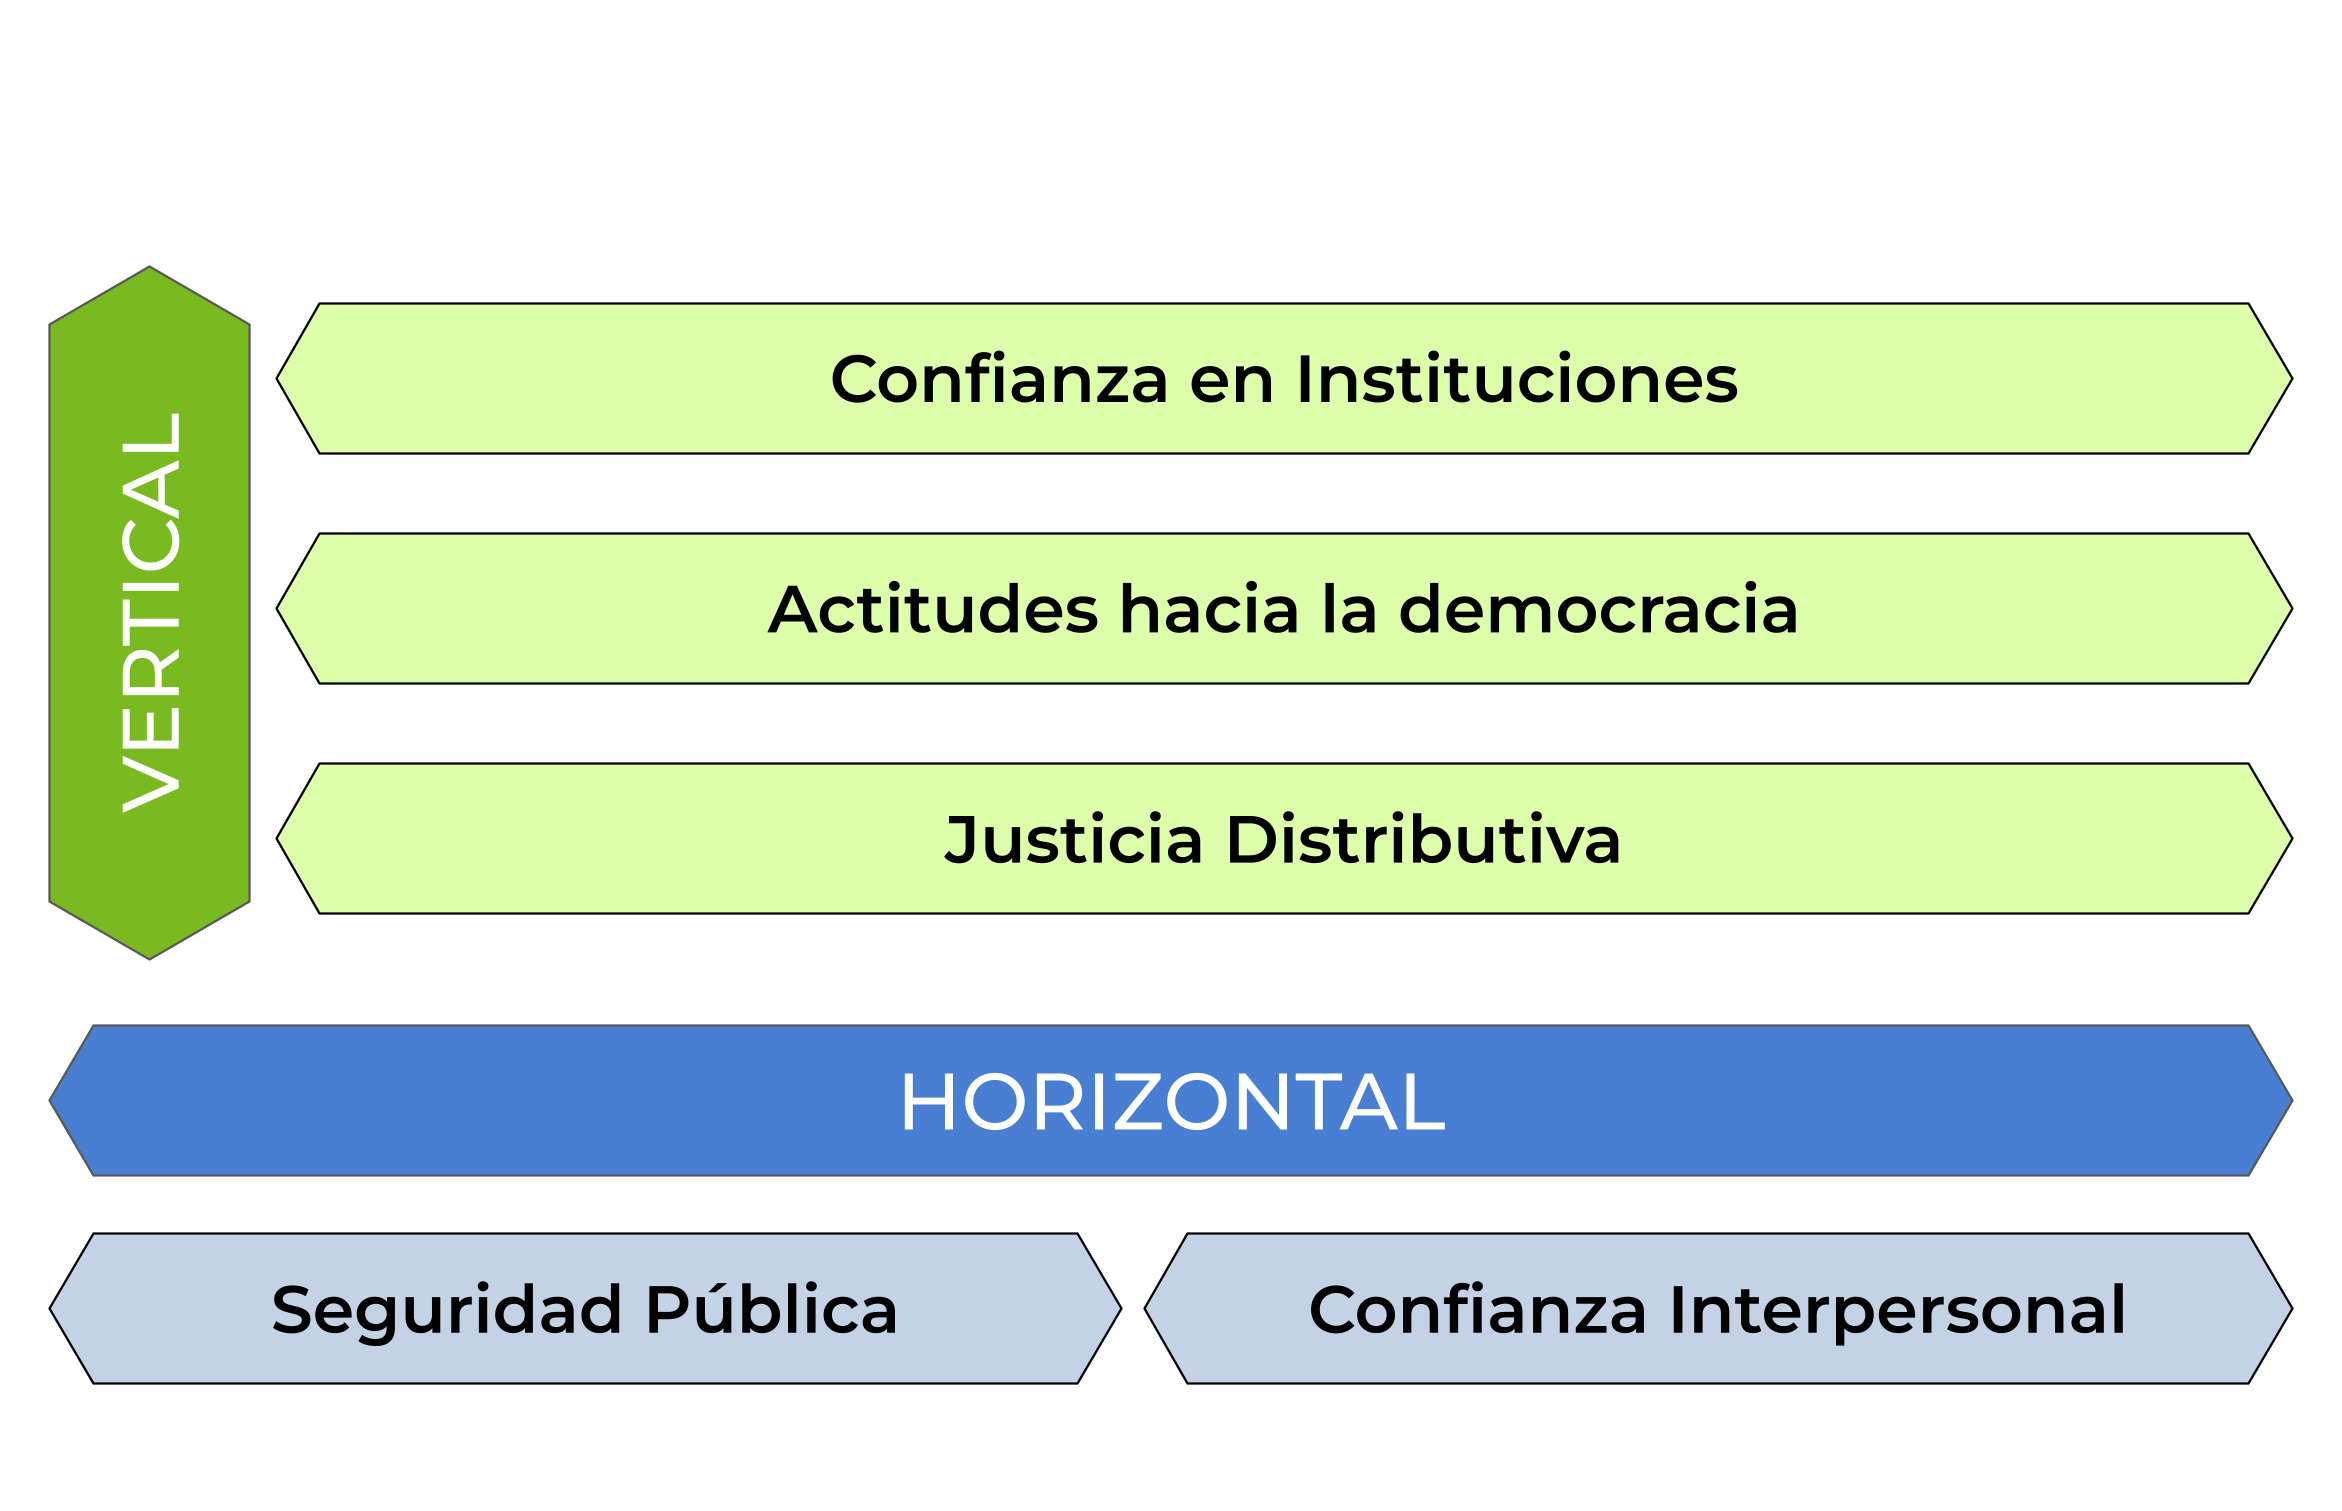
\includegraphics[keepaspectratio]{input/esquema.png}}

}

\caption{\label{fig-modelo}Esquema Conceputal de Cohesión Social}

\end{figure}%

\subsubsection{Análisis Multinivel}\label{anuxe1lisis-multinivel}

Dada la estructura jerárquica de los datos, se estimaron modelos de
regresión multinivel híbridos. Esta técnica permite utilizar datos a
nivel individual para descomponer los efectos a nivel país en sus
componentes entre países (\emph{efectos between}) y dentro de un país en
el tiempo (\emph{efectos within})
(\citeproc{ref-schmidt-catran_random_2016}{Schmidt-Catran y Fairbrother
2016}; \citeproc{ref-fairbrother_two_2014}{Fairbrother 2014}). Los
modelos fueron estimados usando el paquete de R \texttt{lme4}
(\citeproc{ref-bates_fitting_2015}{Bates et~al. 2015}).

El modelo propuesto se podría expresar formalmente como:

\[
y_{jti} = \beta_{0}(t) + \beta_{1}X_{jti} + \gamma_{we}(Z_{jt}-\bar{Z}_{j}) + \gamma_{be}\bar{Z}_{j} + v_j + u_{jt} + e_{jti}
\] El modelo integra 3 niveles con individuos \(i\) anidados en
olas-países \(t\) anidados países \(j\). \(X_{jti}\) representa
variables de nivel individual mientras que \(Z_{jt}\) son variables
contextuales a nivel ola-país. Dado que \(Z_{jt}\) contiene varianza
tanto de nivel 2 como de nivel 3, se descompuso en el promedio de la
variable a lo largo de todas sus olas (\(\bar{Z}_{j}\)) y en la
desviación intra-país en una ola dada (\(Z_{jt}-\bar{Z}_{j}\)). De tal
forma, \(\gamma_{we}\) representa en el efecto \emph{within}, es decir,
el efecto del cambio en un país en el tiempo; mientras que
\(\gamma_{be}\) representa el efecto \emph{between}, es decir, las
diferencias estructurales entre países. Además, \(\beta_{0}(t)\)
controla cambios en el tiempos no explicados por el modelo. Por último,
\(v_j\), \(u_{jt}\) y \(e_{jti}\) representan los errores a nivel país,
ola-país e individual.

\section{Resultados}\label{resultados}

\subsection{Descriptivos}\label{descriptivos}

\begin{figure}[H]

\centering{

\pandocbounded{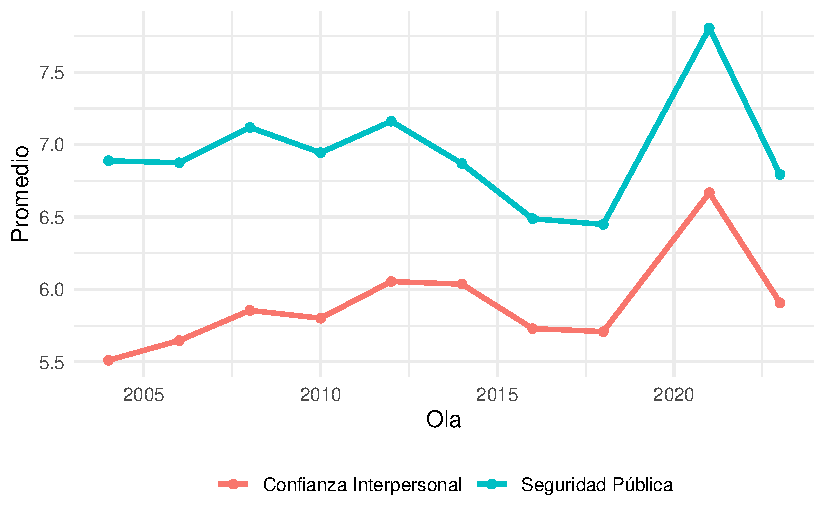
\includegraphics[keepaspectratio]{index_files/figure-pdf/fig-ch-1.pdf}}

}

\caption{\label{fig-ch}Evolución dimensiones Cohesión Horizontal
(2004-2022)}

\end{figure}%

\begin{figure}[H]

\centering{

\pandocbounded{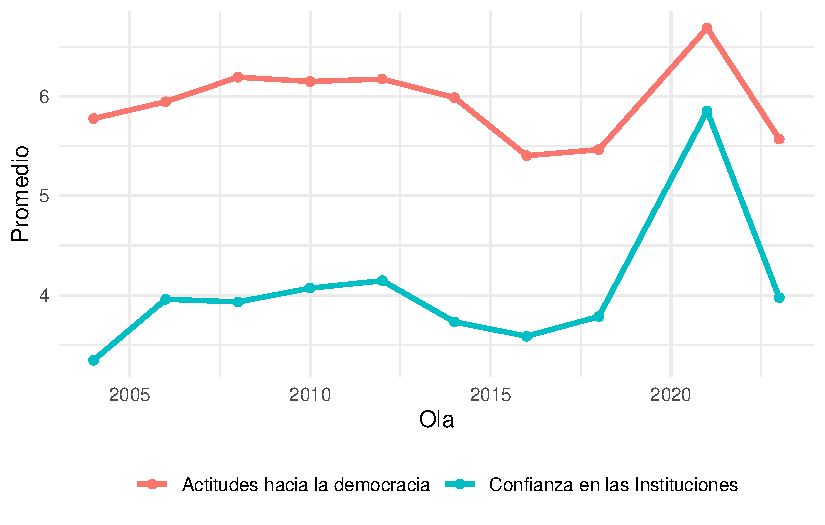
\includegraphics[keepaspectratio]{index_files/figure-pdf/fig-cv-1.pdf}}

}

\caption{\label{fig-cv}Evolución dimensiones Cohesión Vertical
(2004-2022)}

\end{figure}%

\begin{figure}[H]

\centering{

\pandocbounded{\includegraphics[keepaspectratio]{index_files/figure-pdf/fig-correlación-1.pdf}}

}

\caption{\label{fig-correlación}Correlación subdimensiones de la
Cohesión Social}

\end{figure}%

\subsection{Análisis Factorial
Confirmatorio}\label{anuxe1lisis-factorial-confirmatorio-1}

\begin{figure}[H]

{\centering \pandocbounded{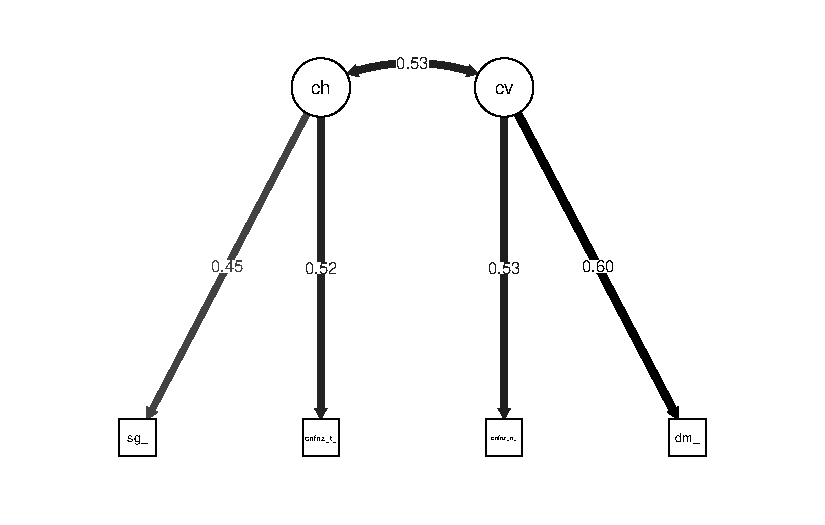
\includegraphics[keepaspectratio]{index_files/figure-pdf/afc-1.pdf}}

}

\caption{Análisis Factorial Confirmatorio Modelo de Medición de Cohesión
Social}

\end{figure}%

Nota. RMSEA = 0.021, CFI = 0.998, Chi-cuadrado = 103, gl = 1, p-valor =
0.

\begin{figure}[H]

\centering{

\pandocbounded{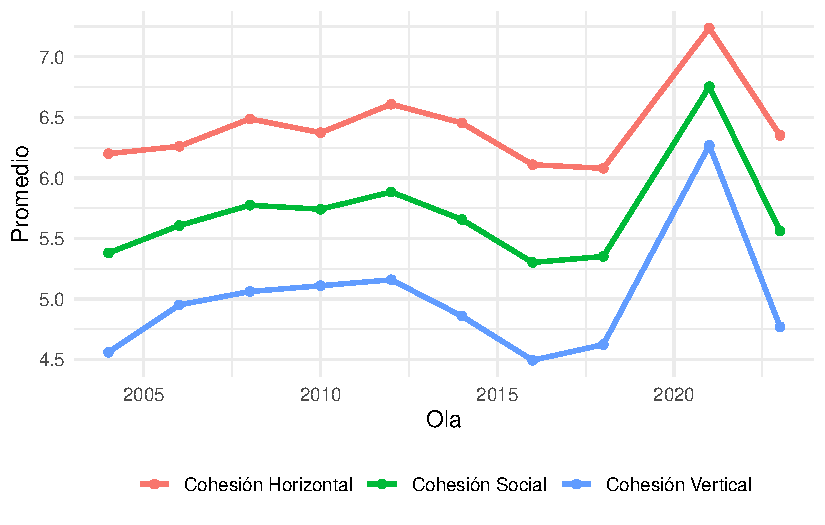
\includegraphics[keepaspectratio]{index_files/figure-pdf/fig-cs-1.pdf}}

}

\caption{\label{fig-cs}}

\end{figure}%

\subsection{Modelos Multinivel}\label{modelos-multinivel}

\begin{table}

\caption{\label{tbl-modelos-horizontal}Modelos para cohesión horizontal}

\centering{

Statistical models

~

Model 1

Model 2

Model 3

(Intercept)

6.48***

6.74***

7.80***

~

(0.15)

(0.16)

(0.53)

factor(ola)2006

-0.03

-0.14

-0.13

~

(0.11)

(0.12)

(0.12)

factor(ola)2008

0.03

-0.20

-0.19

~

(0.11)

(0.13)

(0.13)

factor(ola)2010

-0.04

-0.25

-0.23

~

(0.11)

(0.14)

(0.14)

factor(ola)2012

0.18

-0.12

-0.10

~

(0.11)

(0.15)

(0.15)

factor(ola)2014

0.04

-0.36*

-0.33*

~

(0.11)

(0.16)

(0.17)

factor(ola)2016

-0.27*

-0.70***

-0.66***

~

(0.11)

(0.17)

(0.18)

factor(ola)2018

-0.41***

-0.85***

-0.81***

~

(0.12)

(0.19)

(0.20)

factor(ola)2022

-0.27*

-0.80***

-0.74**

~

(0.11)

(0.22)

(0.23)

pib\_c

~

0.38*

0.47*

~

~

(0.19)

(0.21)

gini\_c

~

-0.01

-0.01

~

~

(0.01)

(0.01)

vdem\_c

~

-1.35*

-0.95

~

~

(0.53)

(0.54)

wgi\_c

~

0.38*

0.20

~

~

(0.18)

(0.19)

mig\_c

~

-0.01

-0.05

~

~

(0.02)

(0.03)

regionCentroamérica

~

~

-0.93

~

~

~

(0.61)

regionEl Caribe

~

~

-1.16

~

~

~

(0.67)

regionAmérica del Sur

~

~

-1.39*

~

~

~

(0.61)

AIC

217.93

182.08

181.24

BIC

254.26

230.87

239.19

Log Likelihood

-97.96

-75.04

-71.62

Num. obs.

201

156

156

Num. groups: pais

25

22

22

Var: pais (Intercept)

0.30

0.19

0.20

Var: Residual

0.09

0.09

0.08

***p \textless{} 0.001; **p \textless{} 0.01; *p \textless{} 0.05

}

\end{table}%

\begin{table}

\caption{\label{tbl-modelos-vertical}Modelos para cohesión vertical}

\centering{

Statistical models

~

Model 1

Model 2

Model 3

(Intercept)

4.52***

4.82***

4.90***

~

(0.16)

(0.16)

(0.50)

factor(ola)2006

0.16

0.00

0.00

~

(0.14)

(0.14)

(0.14)

factor(ola)2008

0.08

-0.23

-0.22

~

(0.14)

(0.15)

(0.15)

factor(ola)2010

0.14

-0.14

-0.13

~

(0.14)

(0.15)

(0.16)

factor(ola)2012

0.28*

-0.25

-0.24

~

(0.14)

(0.16)

(0.17)

factor(ola)2014

0.05

-0.38*

-0.36*

~

(0.14)

(0.17)

(0.18)

factor(ola)2016

-0.21

-0.73***

-0.71***

~

(0.14)

(0.18)

(0.19)

factor(ola)2018

-0.27

-0.81***

-0.79***

~

(0.14)

(0.19)

(0.21)

factor(ola)2022

-0.23

-0.75***

-0.72**

~

(0.14)

(0.22)

(0.24)

pib\_c

~

0.15

0.13

~

~

(0.18)

(0.20)

gini\_c

~

-0.04**

-0.04**

~

~

(0.01)

(0.01)

vdem\_c

~

-3.09***

-3.19***

~

~

(0.56)

(0.60)

wgi\_c

~

0.80***

0.83***

~

~

(0.18)

(0.20)

mig\_c

~

-0.01

-0.01

~

~

(0.02)

(0.03)

regionCentroamérica

~

~

-0.15

~

~

~

(0.57)

regionEl Caribe

~

~

-0.12

~

~

~

(0.62)

regionAmérica del Sur

~

~

-0.06

~

~

~

(0.57)

AIC

290.08

203.33

210.52

BIC

326.41

252.12

268.47

Log Likelihood

-134.04

-85.66

-86.26

Num. obs.

201

156

156

Num. groups: pais

25

22

22

Var: pais (Intercept)

0.31

0.12

0.15

Var: Residual

0.14

0.11

0.11

***p \textless{} 0.001; **p \textless{} 0.01; *p \textless{} 0.05

}

\end{table}%

\phantomsection\label{refs}
\begin{CSLReferences}{1}{0}
\bibitem[\citeproctext]{ref-andrews_welfare_2015}
ANDREWS, RHYS, y SEBASTIAN JILKE. 2015. {«Welfare {States} and {Social
Cohesion} in {Europe}: {Does Social Service Quality Matter}?»}
\emph{Journal of Social Policy} 45 (1): 119-40.
\url{https://doi.org/10.1017/s0047279415000513}.

\bibitem[\citeproctext]{ref-araujo_primer_2022}
Araujo, Kathya, Macarena Orchard, Alejandra Rasse, y Antonio Stecher.
2022. {«Primer {Informe} de {Resultados Encuesta Nacional} de {Autoridad
NUMAAP} 2021»}. Santiago de Chile: NUMAAP.

\bibitem[\citeproctext]{ref-ariely_does_2013}
Ariely, Gal. 2013. {«Does {Diversity Erode Social Cohesion}?
{Conceptual} and {Methodological Issues}»}. \emph{Political Studies} 62
(3): 573-95. \url{https://doi.org/10.1111/1467-9248.12068}.

\bibitem[\citeproctext]{ref-bates_fitting_2015}
Bates, Douglas, Martin Mächler, Ben Bolker, y Steve Walker. 2015.
{«Fitting {Linear Mixed-Effects Models Using} {\textbf{Lme4}}»}.
\emph{Journal of Statistical Software} 67 (1).
\url{https://doi.org/10.18637/jss.v067.i01}.

\bibitem[\citeproctext]{ref-cabib_nuestras_2025}
Cabib, Ignacio, Daniel Miranda, Juan Pablo Ormeño, y Daniela Moyano.
2025. {«{Nuestras Trayectorias. Din{á}micas intra-individuales e
inter-individuales en Chile (2016-2023)}»}.
\url{https://doi.org/10.13140/RG.2.2.23888.62720}.

\bibitem[\citeproctext]{ref-castillo_social_2023}
Castillo, Juan Carlos, Macarena Bonhomme, Daniel Miranda, y Julio
Iturra. 2023. {«Social Cohesion and Attitudinal Changes toward
Migration: {A} Longitudinal Perspective amid the {COVID-19} Pandemic»}.
\emph{Frontiers in Sociology} 7 (enero): 1009567.
\url{https://doi.org/10.3389/fsoc.2022.1009567}.

\bibitem[\citeproctext]{ref-castillo_cohesion_2022}
Castillo, Juan Carlos, Vicente Espinoza, y Emmanuelle Barozet. 2022.
{«{Cohesi{ó}n social en Chile en tiempos de cambio: indicadores,
perfiles y factores asociados}»}.

\bibitem[\citeproctext]{ref-castillo_socialization_2024}
Castillo, Juan Carlos, Mauricio Salgado, Kevin Carrasco, y Andreas
Laffert. 2024. {«The {Socialization} of {Meritocracy} and {Market
Justice Preferences} at {School}»}. \emph{Societies} 14 (11): 214.
\url{https://doi.org/10.3390/soc14110214}.

\bibitem[\citeproctext]{ref-castillo_conceptos_2021}
Castillo, Juan-Carlos, Francisco Olivos, y Julio Iturra. 2021.
{«Conceptos y Medici{ó}n de Cohesi{ó}n Social En Proyectos
Internacionales»}. Documentos de \{\{Trabajo COES\}\} 47. Santiago:
COES.

\bibitem[\citeproctext]{ref-chan_reconsidering_2006}
Chan, Joseph, Ho-Pong To, y Elaine Chan. 2006. {«Reconsidering {Social
Cohesion}: {Developing} a {Definition} and {Analytical Framework} for
{Empirical Research}»}. \emph{Social Indicators Research} 75 (2):
273-302. \url{https://doi.org/10.1007/s11205-005-2118-1}.

\bibitem[\citeproctext]{ref-delhey_social_2018}
Delhey, Jan, Klaus Boehnke, Georgi Dragolov, Zsófia S. Ignácz, Mandi
Larsen, Jan Lorenz, y Michael Koch. 2018. {«Social {Cohesion} and {Its
Correlates}: A {Comparison} of {Western} and {Asian Societies}»}.
\emph{Comparative Sociology} 17 (3-4): 426-55.
\url{https://doi.org/10.1163/15691330-12341468}.

\bibitem[\citeproctext]{ref-delhey_happier_2016}
Delhey, Jan, y Georgi Dragolov. 2016. {«Happier {Together}. {Social
Cohesion} and {Subjective Well-Being} in {Europe}: {HAPPIER
TOGETHER-COHESION AND SWB}»}. \emph{International Journal of Psychology}
51 (3): 163-76. \url{https://doi.org/10.1002/ijop.12149}.

\bibitem[\citeproctext]{ref-delhey_social_2023}
Delhey, Jan, Georgi Dragolov, y Klaus Boehnke. 2023. {«Social {Cohesion}
in {International Comparison}: A {Review} of {Key Measures} and
{Findings}»}. \emph{KZfSS K{ö}lner Zeitschrift f{ü}r Soziologie und
Sozialpsychologie} 75 (S1): 95-120.
\url{https://doi.org/10.1007/s11577-023-00891-6}.

\bibitem[\citeproctext]{ref-dragolov_social_2013}
Dragolov, Georgi, Zsófia Ignácz, Jan Lorenz, Jan Delhey, y Klaus
Boehnke. 2013. {«Social {Cohesion Radar Measuring Common Ground}: {An
International Comparison} of {Social Cohesion Methods Report}»}.

\bibitem[\citeproctext]{ref-fairbrother_two_2014}
Fairbrother, Malcolm. 2014. {«Two {Multilevel Modeling Techniques} for
{Analyzing Comparative Longitudinal Survey Datasets}»}. \emph{Political
Science Research and Methods} 2 (1): 119-40.
\url{https://doi.org/10.1017/psrm.2013.24}.

\bibitem[\citeproctext]{ref-gijsberts_hunkering_2011}
Gijsberts, Mérove, Tom van der Meer, y Jaco Dagevos. 2011.
{«{``{Hunkering Down}''} in {Multi-Ethnic Neighbourhoods}? {The Effects}
of {Ethnic Diversity} on {Dimensions} of {Social Cohesion}»}.
\emph{European Sociological Review} 28 (4): 527-37.
\url{https://doi.org/10.1093/esr/jcr022}.

\bibitem[\citeproctext]{ref-green_social_2011}
Green, Andy, Germ Janmaat, y Helen Cheng. 2011. {«Social {Cohesion}:
{Converging} and {Diverging Trends}»}. \emph{National Institute Economic
Review} 215 (enero): R6-22.
\url{https://doi.org/10.1177/0027950111401140}.

\bibitem[\citeproctext]{ref-janmaat_social_2010}
Janmaat, Jan Germen. 2010. {«Social {Cohesion} as a {Real-life
Phenomenon}: {Assessing} the {Explanatory Power} of the {Universalist}
and {Particularist Perspectives}»}. \emph{Social Indicators Research}
100 (1): 61-83. \url{https://doi.org/10.1007/s11205-010-9604-9}.

\bibitem[\citeproctext]{ref-kaufmann_worldwide_2024}
Kaufmann, Daniel, y Aart Kraay. 2024. {«The {Worldwide Governance
Indicators}»}. Policy \{\{Research Working Paper\}\} WPS10952.
Washington D.C.: World Bank.

\bibitem[\citeproctext]{ref-kustov_diversity_2024}
Kustov, Alexander, y Giuliana Pardelli. 2024. {«Beyond {Diversity}: {The
Role} of {State Capacity} in {Fostering Social Cohesion} in {Brazil}»}.
\emph{World Development} 180 (agosto): 106625.
\url{https://doi.org/10.1016/j.worlddev.2024.106625}.

\bibitem[\citeproctext]{ref-langer_conceptualising_2016}
Langer, Arnim, Frances Stewart, Kristien Smedts, y Leila Demarest. 2016.
{«Conceptualising and {Measuring Social Cohesion} in {Africa}: {Towards}
a {Perceptions-Based Index}»}. \emph{Social Indicators Research} 131
(1): 321-43. \url{https://doi.org/10.1007/s11205-016-1250-4}.

\bibitem[\citeproctext]{ref-lapoplab_americasbarometer_2023}
LAPOP LAb. 2023. {«{AmericasBarometer}»}.

\bibitem[\citeproctext]{ref-maerz_vdemdata_2025}
Maerz, Seraphine F., Amanda B. Esgell, Sebastian Hellemeier, Nina
Illchenko, y Linnea Fox. 2025. {«Vdemdata: {An R} Package to Load,
Explore and Work with the Most Recent {V-Dem} ({Varieties} of
{Democracy}) Dataset.»}

\bibitem[\citeproctext]{ref-meer_ethnic_2014}
Meer, Tom van der, y Jochem Tolsma. 2014. {«Ethnic {Diversity} and {Its
Effects} on {Social Cohesion}»}. \emph{Annual Review of Sociology} 40
(1): 459-78. \url{https://doi.org/10.1146/annurev-soc-071913-043309}.

\bibitem[\citeproctext]{ref-mideso_informe_2020}
Ministerio de Desarrollo Social y Familia. 2020. {«Informe {Final
Consejo Asesor} Para La {Cohesi{ó}n Social}. {Diagn{ó}stico} Para Una
Aproximaci{ó}n a La Cohesi{ó}n Social En {Chile} y Recomendaciones Para
Fortalecer El Aporte de La Pol{í}tica Social»}.

\bibitem[\citeproctext]{ref-njozela_measuring_2016}
Njozela, Lindokuhle, I. Shaw, y J. Burns. 2016. {«Towards Measuring
Social Cohesion in {South Africa}»}.

\bibitem[\citeproctext]{ref-observatoriodecohesionsocial_medicion_2025}
Observatorio de Cohesión Social. 2025. {«Medici{ó}n {Cohesi{ó}n Social
Am{é}rica Latina}»}. Santiago: COES.

\bibitem[\citeproctext]{ref-reeskens_nationalism_2012}
Reeskens, Tim, y Matthew Wright. 2012. {«Nationalism and the {Cohesive
Society}»}. \emph{Comparative Political Studies} 46 (2): 153-81.
\url{https://doi.org/10.1177/0010414012453033}.

\bibitem[\citeproctext]{ref-salazar-xirinachs_repensar_2023}
Salazar-Xirinachs, José Manuel. 2023. {«{Repensar, reimaginar,
transformar: los {``qu{é}''} y los {``c{ó}mo''} para avanzar hacia un
modelo de desarrollo m{á}s productivo, inclusivo y sostenible}»}.
\emph{Revista de la CEPAL} 2023 (141): 11-43.
\url{https://doi.org/10.18356/16820908-2023-141-2}.

\bibitem[\citeproctext]{ref-schmidt-catran_random_2016}
Schmidt-Catran, Alexander W., y Malcolm Fairbrother. 2016. {«The {Random
Effects} in {Multilevel Models}: {Getting Them Wrong} and {Getting Them
Right}»}. \emph{European Sociological Review} 32 (1): 23-38.
\url{https://doi.org/10.1093/esr/jcv090}.

\bibitem[\citeproctext]{ref-somma_paradojas_2015}
Somma, Nicolás M, y Eduardo Valenzuela. 2015. {«Las {Paradojas} de {La
Cohesi{ó}n Social En Am{é}rica Latina}»}. \emph{Revista del CLAD Reforma
y Democracia}, n.º 61: 43-74.

\bibitem[\citeproctext]{ref-stefoni_panorama_2018}
Stefoni, Carolina. 2018. {«{Panorama de la migraci{ó}n internacional en
Am{é}rica del Sur}»}.

\bibitem[\citeproctext]{ref-toppi_guillermo_2018}
Toppi, Hernán Pablo. 2018. {«Guillermo {O}'{Donnell} y Su Aporte al
Desarrollo de La Democracia En {Am{é}rica Latina} Desde La Tercera Ola
de Democratizaci{ó}n»}. \emph{REVISTA IUS} 12 (42).
\url{https://doi.org/10.35487/rius.v12i42.2018.407}.

\bibitem[\citeproctext]{ref-undp_trapped_2023}
United Nations Development Programme. 2023. \emph{Trapped: {High
Inequality} and {Low Growth} in {Latin America} and the {Caribbean}:
{Regional Human Development Report} 2021}. United Nations.
\url{https://doi.org/10.18356/9789210057844}.

\end{CSLReferences}




\end{document}
